\section{Velocity Model of the Vehicle}
In this section the driving part of the vehicle in \chapref{cha:ModelOfVehicle}, \figref{fig:completeMechanicalDiagram} is described and modelled. The following subsections will therefore focus on getting the relation between the input voltage applied to the motor and the system's output velocity when applied a specific input voltage. The schematic in \chapref{cha:ModelOfVehicle}, \figref{fig:completeMechanicalDiagram} is reduced to the following \figref{fig:vehicleDescriptionDriveTrainBlackBox}.

\begin{figure}[H]
	\centering
	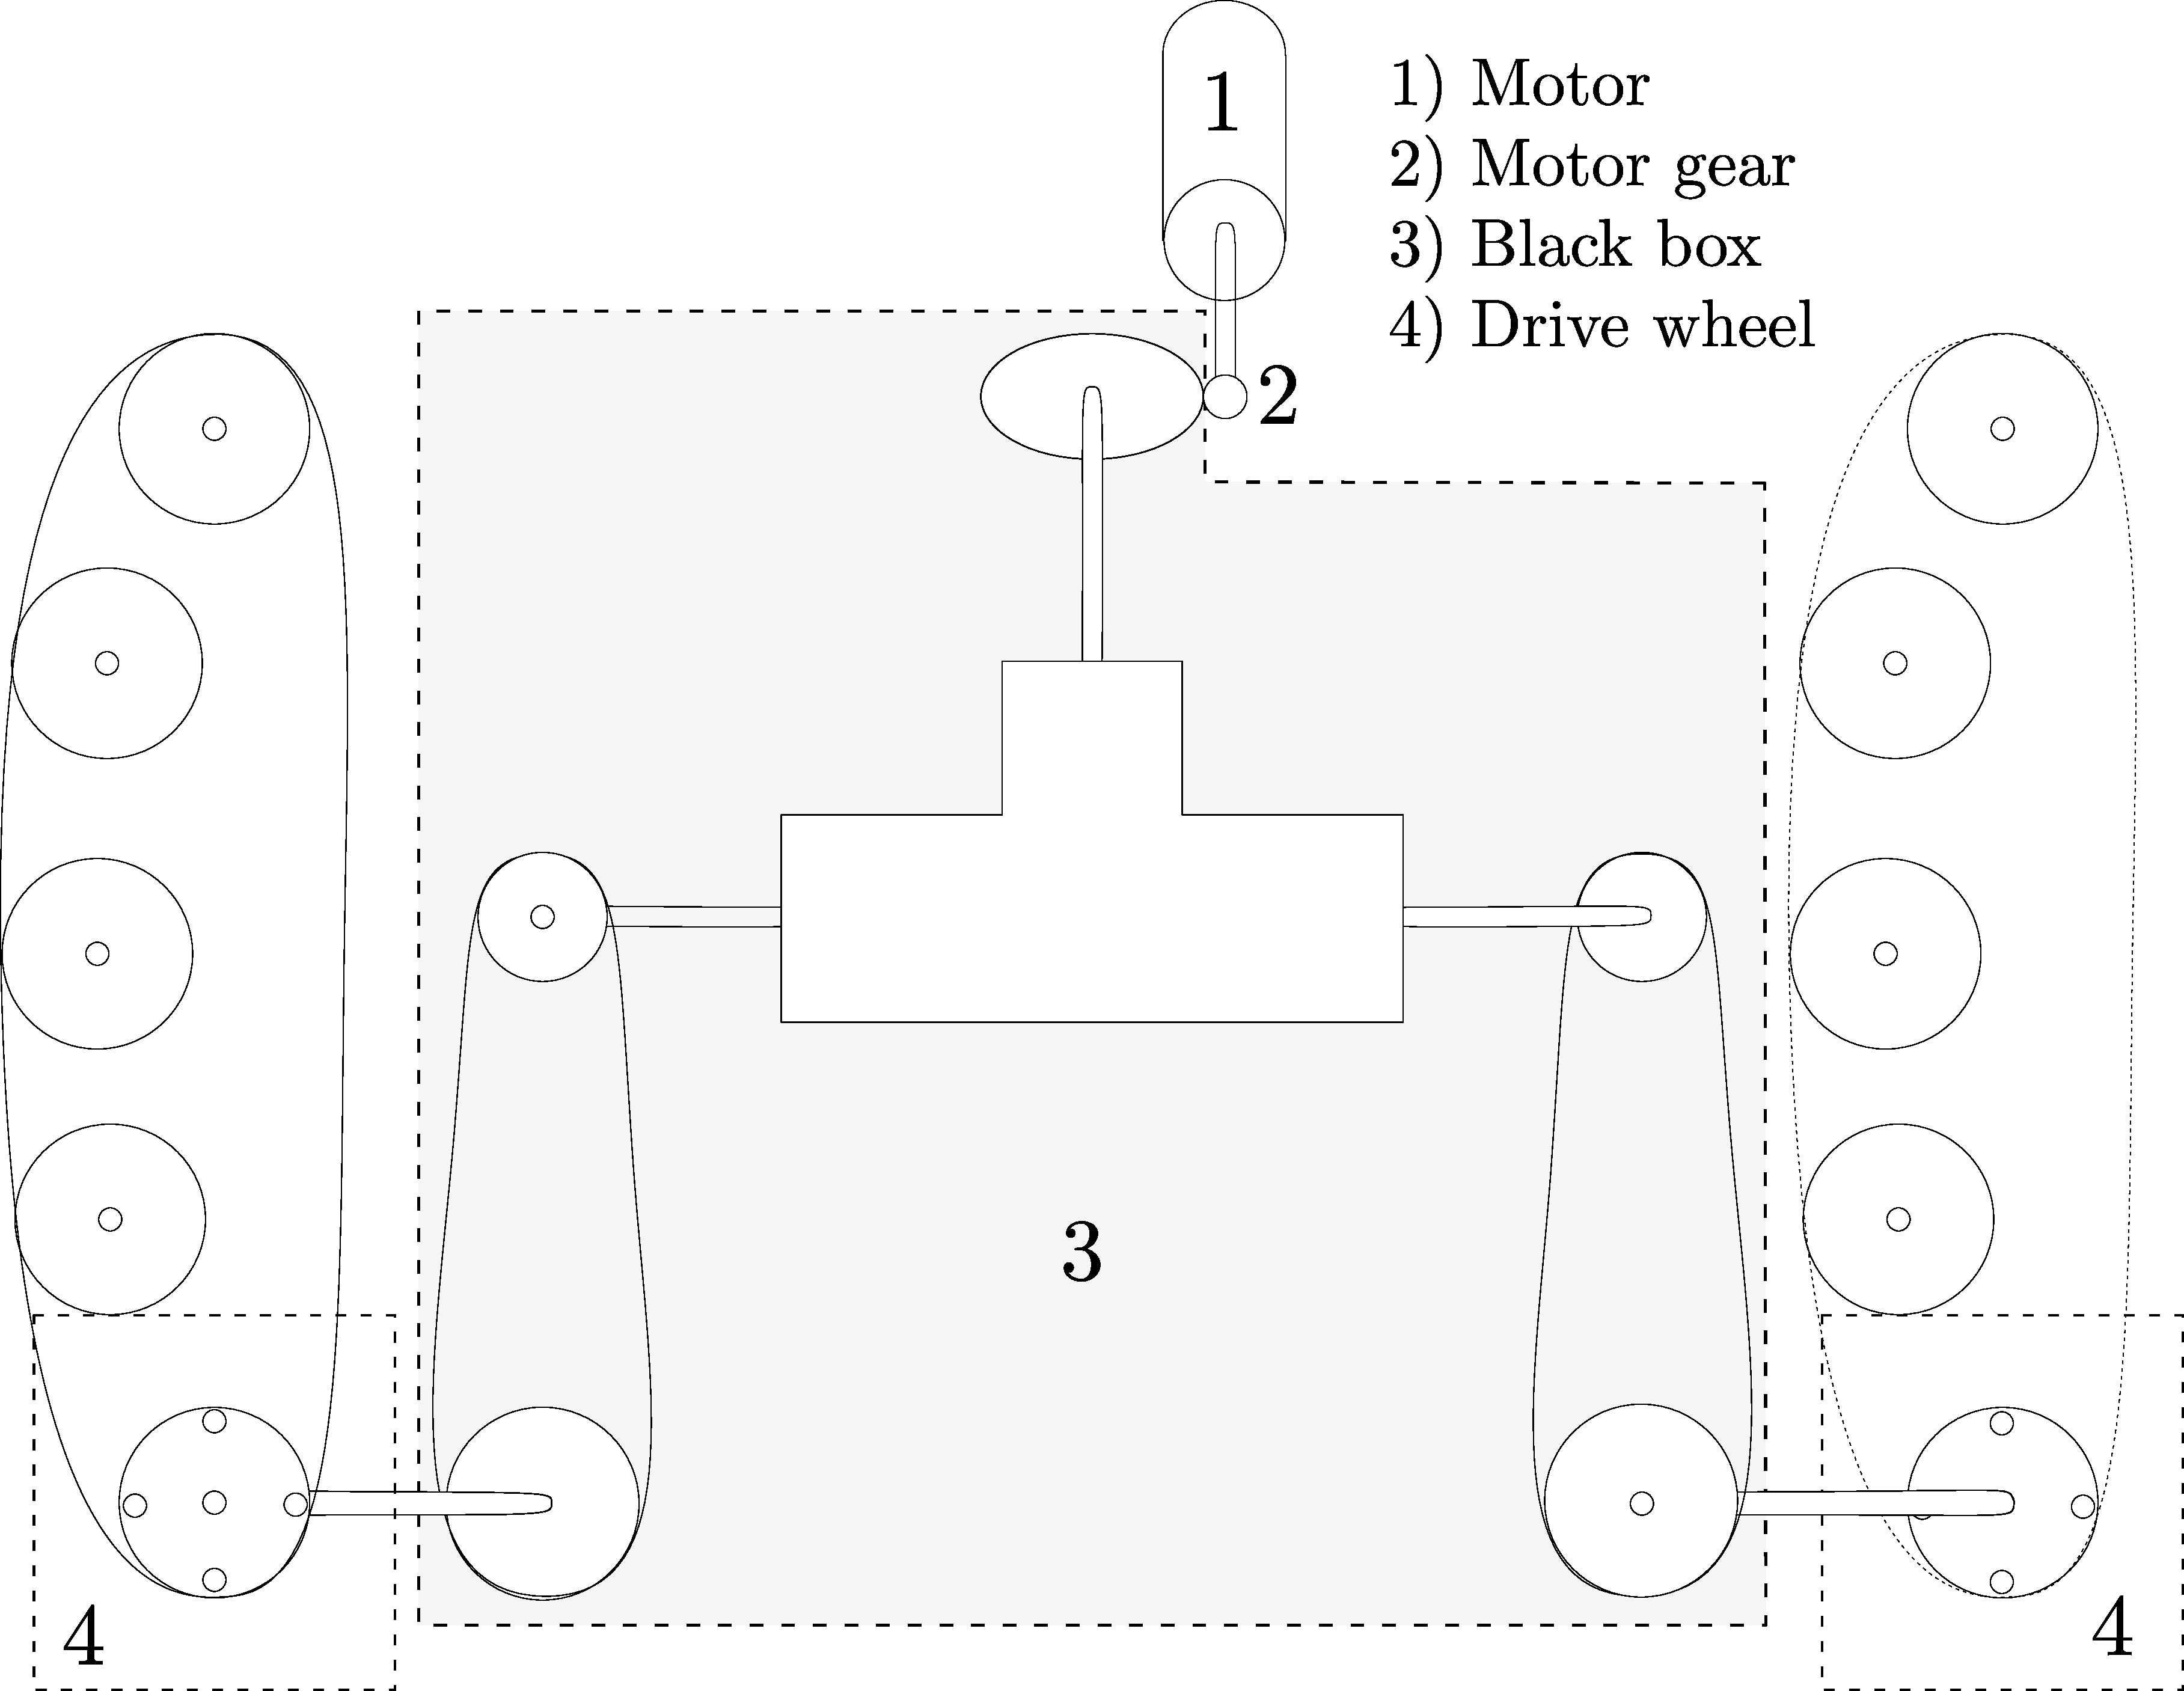
\includegraphics[scale=0.2]{figures/vehicleDescriptionDriveTrainBlackBox.pdf}
	\caption{A mechanical diagram of the driving part of the system}
	\label{fig:vehicleDescriptionDriveTrainBlackBox}
\end{figure}

The system on \figref{fig:vehicleDescriptionDriveTrainBlackBox} is expanded into four different parts to facilitate the modeling process.\\
The first part is the motor itself which is the actuator and is controlled by an input voltage. The mechanical work -produced thereby in the form of a torque- is translated onto the motor shaft and to the motor gear, which is the second part.
The third part consists of the largest part of the drivetrain, from and excluding the motor gear to the gear that sits on the same shaft as the drive wheel. These mechanical elements are made up into a single black box, which is named drivetrain gear hereafter.
The last part describes the conversion from the rotary movement of the drive wheel to the translational movement of the vehicle.

The velocity model of the vehicle is built in two main steps in the following subsections. The first step describes the motor's electrical behavior in response to an input voltage. In a second step, a model of the vehicle's velocity is made from the parts $2$ to $4$ in response the motor's torque. These two subsections are derived by only considering the parameters affecting the vehicle when it is driving in a straight line. Thus, the the two belts are supposed to have the exact same velocity, in this first model.

In the following subsection the motor behavior is modelled.